\tikzset{
	nicebox/.style={draw,rounded corners,color=uofgsandstone,fill=uofgsandstone!10,dashed},
	nfbox/.style={draw,rounded corners,color=uofgsandstone,fill=uofgsandstone!5},
	nfbox2/.style={nfbox, fill=uofgsandstone!1},
	gpath/.style={color=uofgheather,thick},
	usepath/.style={color=uofgmocha,thick},
	daemonbox/.style={draw, rounded corners, fill=white,align=center,},
	authbox/.style={draw, rounded corners, fill=uofgpumpkin!30, align=center,},
	client-authbox/.style={authbox,minimum width=1.8cm,rotate=90},
	authflow/.style={color=uofgthistle,thick},
	normflow/.style={color=uofgpillarbox,thick,dash dot},
	readflow/.style={color=uofgcobalt,thick,dash dot},
}

\begin{tikzpicture}
\draw[nfbox, opacity=0.3] (-3.0,-1.5) rectangle ++(7,3.2);
\draw[nfbox2] (-2.9,-1.4) rectangle ++(7,3.2);
\draw[nfbox] (-2.8,-1.3) rectangle ++(7,3.2);
	
\node (test) {
	\begin{tikzpicture}
	\node (name) {
\includegraphics[keepaspectratio,width=1em]{images/ebpf} \textbf{NF \emph{a}}};
	
	\node[draw, rectangle, align=left] (b1) at ($(name) + (1, -0.75)$) {\mintinline{rust}|nf(ctx.body)|};
	\node[draw, rectangle, align=left] (b2) at ($(b1) + (0,-0.8)$) {Get action};
%	\node[draw, rectangle, align=left] (b3) at ($(b2) + (0,-0.55)$) {Write ID};
%	\node[draw, rectangle, align=left] (b4) at ($(b3) + (0,-0.55)$) {Redirect to \afxdp{}};

	\node[draw, rectangle, align=left] (b3) at ($(b2) + (0.75,-1)$) {Write IDs};
	\node[draw, rectangle, align=left] (b4) at ($(b3) + (2.75,0)$) {Redirect to \afxdp{}};
	
	\node (tab) at ($(b1) + (3.5, -0.25)$) {
		\resizebox{3cm}{!}{\begin{tabular}{ccc}
			\toprule
			Result $\circledast$ & Action & \texttt{PROG}\\
			\midrule
			0 & \texttt{Tx} & --- \\
			1 & \texttt{Call} & NF \emph{b} \\
			2 & \texttt{Upcall} & --- \\
			\bottomrule
		\end{tabular}}
	};

	\draw[->, authflow] (b1.south west) to[out=210,in=180] node[midway, left, xshift=0.05cm, yshift=0.3cm] {$\circledast$} (b2.west);
	\draw[->, authflow] (b2.south) to[out=250,in=160] node[midway, right, yshift=0.15cm] {\texttt{Upcall}} (b3.west);
	\draw[->, authflow] (b3.east) -- (b4.west);
	\draw[->, authflow] (b2.south) to[out=250,in=0] node[midway, right, yshift=0.15cm, xshift=-2cm] {\texttt{Tx, Drop}} ($(b2.south) + (-2.5, -1)$);
	\draw[->, authflow] (b2.south west) to[out=210,in=180] node[midway, below, align=center, xshift=-0.5cm, yshift=0.2cm] {\texttt{Call}\\\texttt{NF}} ($(name.west) + (-0.25, 0)$);
	\draw[->, authflow] (b4.south) to[out=270,in=0] node[midway, below, align=center, xshift=-1cm, yshift=0.15cm] {\texttt{Tx}} ($(b4.south) + (-1, -0.5)$);
	
	\draw[->, readflow] (tab.west) to node[midway, below, xshift=0.4cm, yshift=0.1cm] {\footnotesize\texttt{get($\circledast$)}} (b2.east);	
	\end{tikzpicture}
};

\node (xsks) at (5.5,0.25) {
	\begin{tikzpicture}
		\node[opacity=0.1] at (0.3,-0.3) {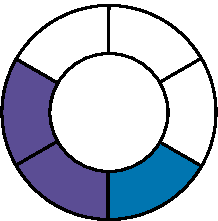
\includegraphics[keepaspectratio,width=3em]{images/ringbuf}};
		\node[opacity=0.25] at (0.2,-0.2) {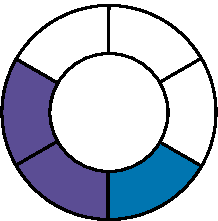
\includegraphics[keepaspectratio,width=3em]{images/ringbuf}};
		\node[opacity=0.5] at (0.1,-0.1) {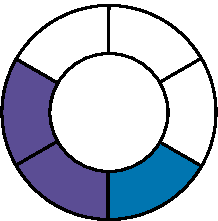
\includegraphics[keepaspectratio,width=3em]{images/ringbuf}};
		\node at (-0,0) {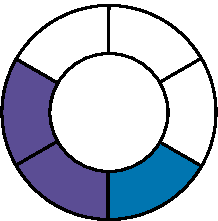
\includegraphics[keepaspectratio,width=3em]{images/ringbuf}};
	\end{tikzpicture}
};

\node[align=center] (xsk-lab) at ($(xsks) + (-0.1,-1.2)$) {\afxdp\\Sockets (XSKs)};

\node[color=uofgrust] (xdp-text) at ($(test) + (-0.9,2.3)$) {\large\texttt{\textbf{Entry:} XDP hook}};
\draw[->, authflow] (xdp-text) to[out=-45,in=45] ($(xdp-text) + (0, -1)$);

\draw[->, readflow] ($(xsks.west) + (0.1,0)$) to node[midway, below, xshift=-1.4cm, yshift=0cm] {\footnotesize\texttt{get(rand())}} ($(xsks.west) + (-0.9,-0.9)$);
\end{tikzpicture}